\chapter{Isoterme}
%===============================================================================================
\section{Isoterma B.E.T.}
L'isoterma B.E.T (sviluppata da 
Brauneuer\footnote{Dire chi �...}, 
Emmett\footnote{Emmett, Paul Hugh (Portland 1900 - 1985), Chimico americano } e 
Teller\footnote{Teller, Edward (Ungheria 1908 - America 2003), Fisico nucleare}) 
si basa su di un approccio di tipo statistico, in cui una superficie che espone dei punti di adsorbimento (siti) viene coperta da uno o pi� strati di molecole di gas, come � visibile in \figurename~\ref{fig:BET:SchemaMolecole}

\begin{figure}[htbp]
	\centering
		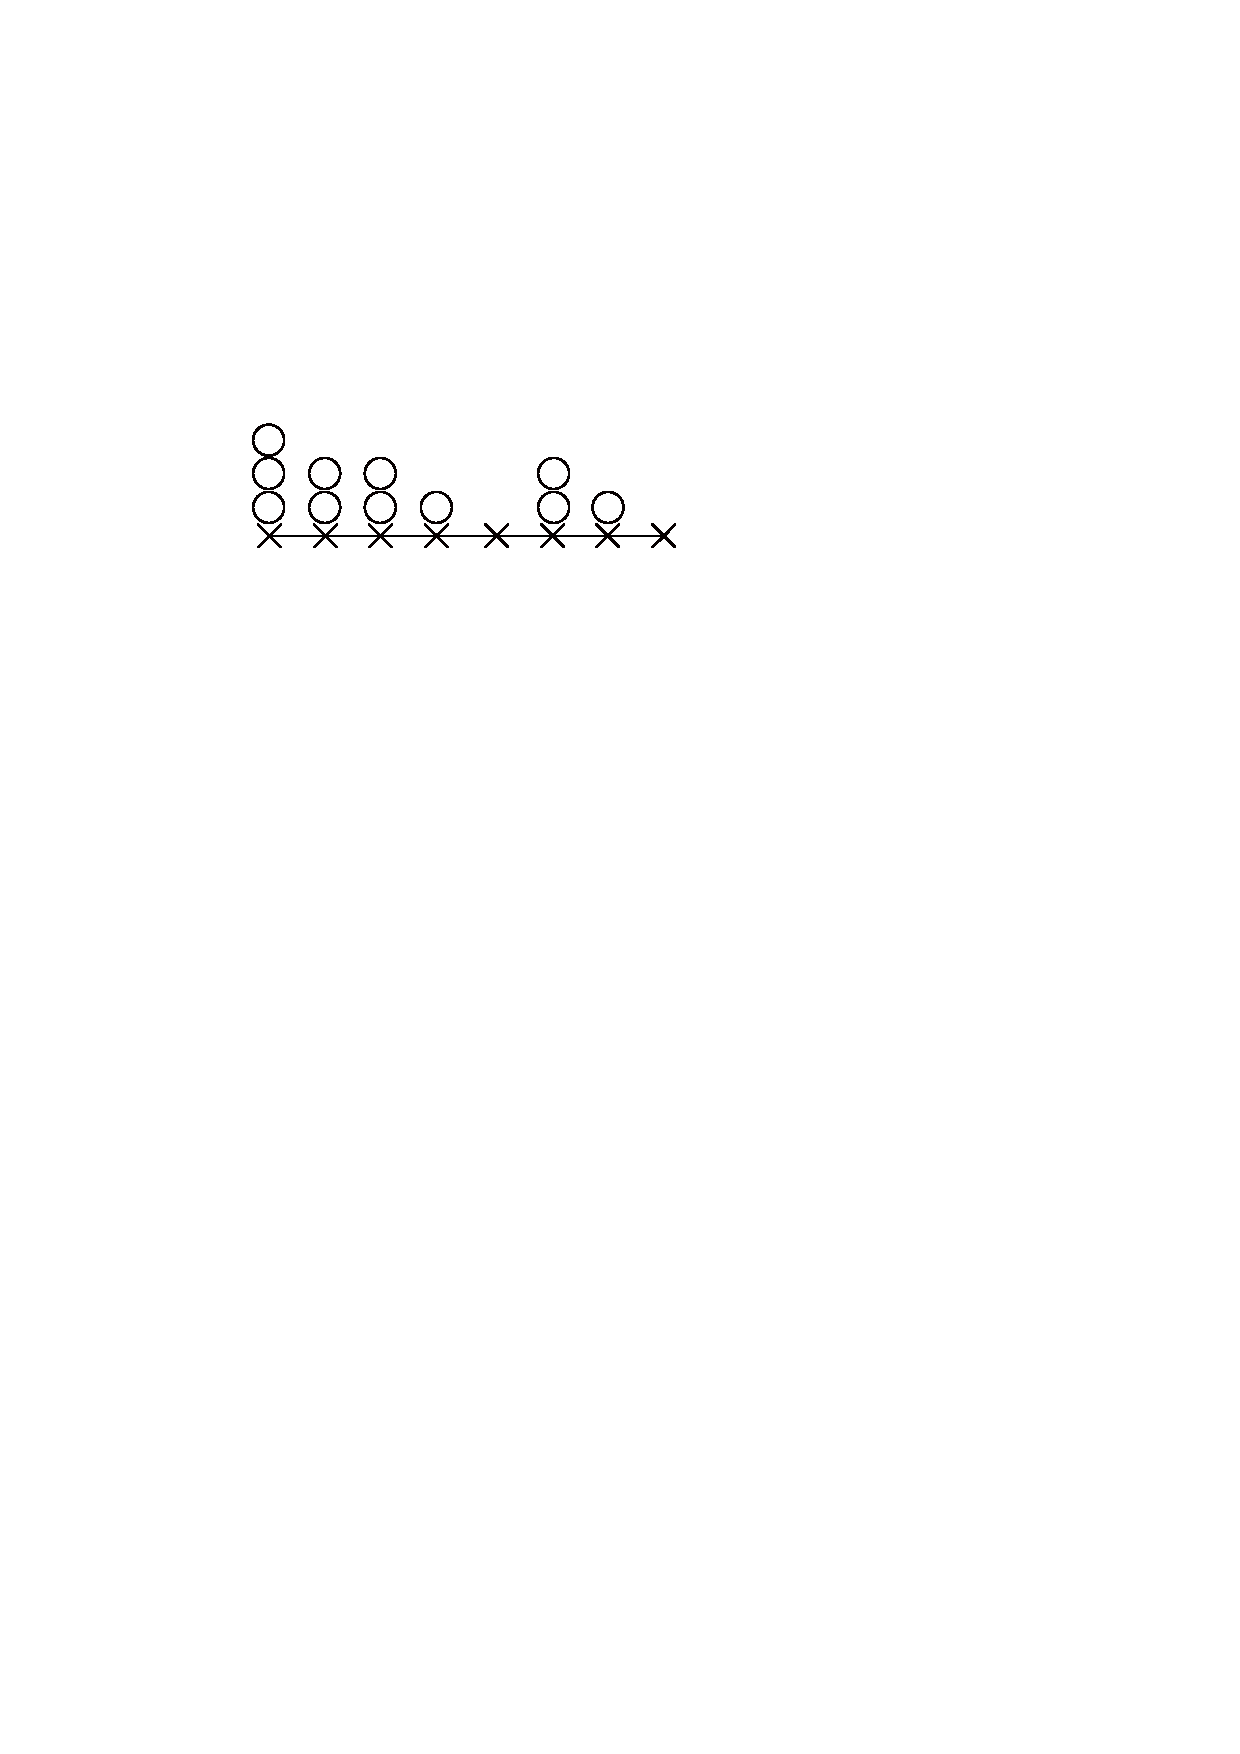
\includegraphics[width=0.50\textwidth]{image/BETSchemaMolecole.pdf}
	\caption{Schema rappresentativo della teoria alla base dell'\textit{isoterma B.E.T.}}
	\label{fig:BET:SchemaMolecole}
\end{figure}

Utilizzeremo $\vartheta_i$ per indicare la frazione dei siti ricoperti da $i$ strati di molecole, quindi sar� anche verificato:
\begin{equation}
	\vartheta_0 + \sum^\infty_{i=1}\vartheta_i = 1
	\label{eq:SommaEpsilon}
\end{equation}

Il simbolo $\sigma$ rappresenta il numero di molecole adsorbite per unit� di area e pu� essere determinato come:
\begin{equation}
	\sigma = \sum^n_{i=1}\vartheta_i \cdot \sigma_m \cdot i
	\label{eq:Sigma}
\end{equation}
dove $\sigma_m$ indica il numero di siti per unit� di area presenti sulla superficie.

Consideriamo ora le reazioni di adsorbimento dei vari strati:
\begin{align}
	G + S_0 \underset{r_{des^1}}{\overset{r_{ad^1}}{\rightleftharpoons}} S_1 \\
	G + S_1 \underset{r_{des^2}}{\overset{r_{ad^2}}{\rightleftharpoons}} S_2 \\
	\dots  \\
	G + S_{n-1} \underset{r_{des^n}}{\overset{r_{ad^n}}{\rightleftharpoons}} S_n
	\label{reaz:Adsorbimento}
\end{align}
essendo per definizione
\begin{align}
	r_{ads}^i = K_{ads}^i \cdot G \cdot \vartheta_{1-i} \cdot \sigma_m	\\
	r_{des}^i = K_{des}^i \cdot \vartheta_{i} \cdot \sigma_m
	\label{eq:VelAdDes}
\end{align}
Che scritte per la serie di reazioni prima considerate porta ad avere,
considerando di essere all'equalibrio ($r_{ads}^i = r_{des}^i$), ed 
essendo la concentrazione del gas $G = \frac{n}{V}=\frac{P}{R T}$:
\begin{align}
	K_{ads}^{1} \cdot \frac{P}{R T} \cdot \vartheta_{0} \cdot \sigma_m	& =  K_{des}^{1} \cdot \vartheta_{1} \cdot \sigma_m \\
	K_{ads}^{2} \cdot \frac{P}{R T} \cdot \vartheta_{1} \cdot \sigma_m	& =  K_{des}^{2} \cdot \vartheta_{3} \cdot \sigma_m \\
	\dots \\
	K_{ads}^{\infty} \cdot \frac{P^0}{R T} \cdot \sigma_m	& =  K_{des}^{\infty} \cdot \sigma_m
	\label{eq:EquilAdsDes}
\end{align}
L'ultima equazione � ottenuta dal fatto che, quando sulla superficie vi � un film di liquido, 
la pressione � pari alla tensione di vapore e i gradi di ricoprimento possono essere ritenuti 
unitari.

Le costanti di adsorbimento possono essere ritenute costanti, inquanto ci si trova a T basse 
(liquefazione di gas), quindi l'energia cinetica delle molecole � bassa e tutte le particelle 
gassose che raggiungono la superficie vi aderiscono. \\
Le costanti di desorbimento, invece, possono essere ritenute costanti solo per gli strati superiori
perch� non risentono delle interazioni con gli atomi vicini, quindi:
\begin{align}
	K_{ads}^{1} = K_{ads}^{2} = K_{ads}^{3} = \dots = K_{ads}^{n} = K_{ads}\\
	K_{des}^{1} \neq K_{des}^{2} = K_{des}^{3} = \dots = K_{des}^{n} =K_{des}
	\label{eq:CostEqAdsDes}
\end{align}

Dividiamo ora le costanti di equilibrio del primo e dell'$i$-esimo strato per le equazioni di 
equilibrio dello strato $\infty$ (equazioni \ref{eq:EquilAdsDes}) ottenendo:
\begin{align}
	\frac{K_{ads} \cdot \frac{P}{R T} \cdot \vartheta_{0} \cdot \sigma_m}{K_{ads} \cdot \frac{P^0}{R T} \cdot \sigma_m} = &
	\frac{K_{des}^{1} \cdot \vartheta_{1} \cdot \sigma_m}{K_{des} \cdot \sigma_m} & \Longrightarrow &
	\frac{P}{P^0} \cdot \vartheta_0 = \frac{K_{des}^1}{K_{des}} \cdot \vartheta_1 \\
	\frac{K_{ads} \cdot \frac{P}{R T} \cdot \vartheta_{i-1}}{K_{ads} \cdot \frac{P^0}{R T}} = &
	\frac{K_{des} \cdot \vartheta_{i} \cdot \sigma_m}{K_{des} \cdot \sigma_m} & \Longrightarrow &
	\frac{P}{P^0} \cdot \vartheta_{i-1} = \vartheta_{i}
	\label{eq:RappEqui}
\end{align}

Sostituendo il valore di $\vartheta_{i-1}$ con quello di ricavato da $\vartheta_{i-2}$ e
 proseguendo cos� fino a $1$ otterremmo:
\begin{align}
	\vartheta_i = \left( \frac{P}{P^0}\right)^{i-1} \cdot \vartheta_1 = x^{i-1} \cdot \vartheta_1
	\label{eq:EpsilonI}
\end{align}
avendo sostituito $x = \frac{P}{P^0}$. 
Ricavando il valore di $\vartheta_1$ dall'equilibrio (equazione \ref{eq:EquilAdsDes}) 
\begin{align}
	\vartheta_1 = \frac{K_{ads}}{K_{des}^1} \frac{P}{R T} \vartheta_0 
	\label{eq:Epsilon1Equil}
\end{align}
Che sostituita nell'equazione \ref{eq:EpsilonI} porta a:
\begin{align}
	\vartheta_i = \left( \frac{P}{P^0}\right)^{i-1} \cdot \frac{K_{ads}}{K_{des}^1} \frac{P}{R T} \vartheta_0
	\label{eq:EpsilonIEqu}
\end{align}
Moltiplicando e dividendo per $P^0$ e ricordando il significato di $x$ otteniamo:
\begin{align}
	\vartheta_i = \left( \frac{P}{P^0}\right)^{i-1} \cdot \frac{K_{ads}}{K_{des}^1} 
							\frac{P}{R T} \vartheta_0 \cdot \frac{P^0}{P^0} =
							\frac{K_{ads}}{K_{des}^1} \frac{P^0}{R T} x^i \cdot \vartheta_0 =
							C \cdot x^i \cdot \vartheta_0
	\label{eq:EpsilonIFin}
\end{align}
Avendo accorpato in una costante i termini fissi, ovvero $C = \frac{K_{ads}}{K_{des}^1} \frac{P^0}{R T}$

Sostituendo il risultato ottenuto (equazione \ref{eq:EpsilonIFin}) nelle equazioni \ref{eq:SommaEpsilon} e \ref{eq:Sigma} otteniamo:
\begin{equation}
	\vartheta_0 + \sum^\infty_{i=1}\left(C \cdot x^i \cdot \vartheta_0\right) = 1
	\label{eq:SommaEpsilonSost}
\end{equation}
e
\begin{equation}
	\sigma = \sum^n_{i=1}\left(C \cdot x^i \cdot \vartheta_0 \cdot \sigma_m \cdot i\right)
	\label{eq:SigmaSost}
\end{equation}

Il rapporto tra i due termini diventer�:
\begin{equation}
	\frac{\sigma}{1} = 
	\frac	{\sum^n_{i=1}\left(C \cdot x^i \cdot \vartheta_0 \cdot \sigma_m \cdot i\right)}
				{\vartheta_0 + \sum^\infty_{i=1}\left(C \cdot x^i \cdot \vartheta_0\right)}
	\label{eq:RapSigmaUpsilon}
\end{equation}

Le due sommatorie convergono per $\left|x\right| < 1$, infatti:
\begin{equation}
	\sum^{\infty}_{i=1} i \cdot x^i = \frac{x}{(1-x)^2}
	\label{eq:ConvSum1}
\end{equation}
\begin{equation}
	\sum^{\infty}_{i=1} x^i = \sum^{\infty}_{i=1} x^i - 1 = \frac{x}{1-x}
	\label{eq:ConvSum2}
\end{equation}

Note queste caratteristiche delle sommatorie, e tornando all'equazione \ref{eq:RapSigmaUpsilon} otteniamo:
\begin{equation}
	\sigma = 
	\frac	{C \cdot \vartheta_0 \cdot \sigma_m  \frac{x}{(1-x)^2}}
				{\vartheta_0 + \vartheta_0 \cdot C \cdot \frac{x}{1-x}} =
				\frac	{C \cdot \sigma_m  \frac{x}{(1-x)^2}}
							{1 + C \cdot \frac{x}{1-x}} 
	\label{eq:RapSigmaUpsilonSum}
\end{equation}
Che riarrangiando permettono di ottenere:
\begin{equation*}
	\left[ 1 + C \cdot \frac{x}{1-x} \right] \frac{1}{C \cdot \sigma_m} = 
	\frac{1}{\sigma} \cdot \frac{x}{(1-x)^2}
\end{equation*}
\begin{equation*}
	\left[ 1 + C \cdot \frac{x}{1-x} \right] \frac{1}{C \cdot \sigma_m} \cdot (1-x) = 
	\frac{1}{\sigma} \cdot \frac{x}{(1-x)}
\end{equation*}
\begin{equation*}
	\left[ 1 - x + C \cdot x \right] \frac{1}{C \cdot \sigma_m} = 
	\frac{1}{\sigma} \cdot \frac{x}{(1-x)}
\end{equation*}
\begin{equation}
	\frac{1}{C \cdot \sigma_m} + x \cdot \frac{C - 1}{C \cdot \sigma_m} = 
	\frac{1}{\sigma} \cdot \frac{x}{(1-x)}
	\label{eq:RapSigmaUpsilonSumRiarr}
\end{equation}
Ricordando il significato di $x$ e sapendo che $\frac{\sigma}{\sigma_m} = \frac{V_{ads}}{V_m}$
dall'equazione precedente otteniamo:
\begin{equation}
	\frac{1}{C \cdot \sigma_m} + \frac{P}{P^0} \cdot \frac{C - 1}{C \cdot \sigma_m} =
	\frac{P}{P^0} \cdot \frac{\frac{P}{P^0}}{1-\frac{P}{P^0}} \cdot \frac{1}{\sigma_m \cdot \frac{V_{ads}}{V_m}} =
	\frac{1}{C \cdot \sigma_m} + \frac{P}{P^0} \cdot \frac{C -1}{C \cdot \sigma_m}
	\label{eq:RapSigmaUpsilonSumRiarrFin}
\end{equation}
che linearizzata ci permette di ottenere:
\begin{equation}
	\frac{P}{P-P^0} - \frac{1}{V_{ads}} = 
	\frac{1}{C \cdot V_{ads}} + \frac{P^0}{P} \cdot \frac{C - 1}{C \cdot V_m}
	\label{eq:BETLinearizzata}
\end{equation}
Tramite prove sperimentali � possibile ricavare $C$ e $V_m$ e di conseguenza l'equazione � completata e permette di correlare il volume adsorbito ($V_{ads}$) con la pressione del gas ($P$).
%================================================================================================
\section{Isoterma di Langmuir}
Indichiamo con $^*$ la specie adsorbita, e ricordando l'equazione \ref{eq:SommaEpsilon}, introduciamo la variabile $\Gamma^0$ che rappresenta la concentrazione totale dei siti superficiali, � quindi evidente che:
\begin{equation}
	C_i^{*} = \vartheta_i^{*} \cdot \Gamma^0
	\label{eq:ConcStar}
\end{equation}
\begin{equation}
	\sigma = \vartheta_i \cdot \Gamma^0
	\label{eq:ConcSpecie}
\end{equation}
dove $C^{*}$ indica la concentrazione della specie $i$-esima adsorbita e con $\sigma$ la concentrazione dei siti liberi.
Sar� dunque vero anche:
\begin{equation}
	\sigma + \sum_{i=1}^{NS} C_i^{*} = \Gamma^0
	\label{eq:ValGamma0}
\end{equation}
dove $NS$ � il numero di specie che possono essere adsorbite.

Dividendo ambo i membri dell'equazione precedente per $\Gamma^0$ � evidente che:
\begin{equation}
	\frac{\sum_{i=1}^{NS}C_i^{*}}{\Gamma^0} + \frac{\sigma}{\Gamma^0} = \frac{\Gamma^0}{\Gamma^0} =1
	\label{eq:GammaSuGamma}
\end{equation}
e per le equazioni \ref{eq:ConcStar} e \ref{eq:ConcSpecie} anche:
\begin{equation}
	\sum_{i=1}^{NS} \vartheta_i^{*} + \vartheta_i = 1
	\label{eq:SommaUpsilon}
\end{equation}

Scrivendo la generica reazione di adsorbimento e desorbimento abbiamo:
\begin{equation}
	A + \sigma \stackrel{K_{ads}}{\rightarrow} A^{*}
	\label{eq:RxnAds}
\end{equation}
\begin{equation}
	A^{*} \stackrel{K_{des}}{\rightarrow} A + \sigma
	\label{eq:RxnAds2}
\end{equation}
le cui velocit� risulteranno, rispettivamente:
\begin{equation}
	r_{ads} = K_{ads} \cdot C_{A} \cdot C_{\sigma} 
	\label{eq:VelRxnAds}
\end{equation}
\begin{equation}
	r_{des} = K_{des} \cdot C_{A^{*}} 
	\label{eq:VelRxnAds2}
\end{equation}

Applicando il P.S.S.A. sulle specie superficiali abbiamo:
\begin{equation}
	\frac{\partial C_{A^{*}}}{\partial t} = 0
	\label{eq:PSSAAStar}
\end{equation}
\begin{equation}
	\frac{\partial C_{\sigma}}{\partial t} = 0
	\label{eq:PSSACSigma}
\end{equation}
ma anche, considerando una sola specie che si adsorbe:
\begin{equation}
	C_{A^{*}} + C_{\sigma} = \Gamma^0
	\label{eq:SitiOccupati}
\end{equation}
come conseguenza dell'equazione \ref{eq:PSSAAStar} si ha $r_{ads} = r_{des}$ ed esplicitandole:
\begin{equation}
	\left\{
		\begin{array}{l}
			K_{ads} \cdot C_A \cdot C_{\sigma} = K_{des} \cdot C_{A^{*}} \\
			C_{A^{*}} + C_{\sigma} = \Gamma^0
		\end{array}
	\right.
	\label{eq:VelRxnEquil}
\end{equation}
Ricavando $C_{A^{*}}$ dal sistema di equazioni \ref{eq:VelRxnEquil} abbiamo:
\begin{equation}
	C_{A^{*}} = \Gamma^0 - C_{\sigma} = \frac{K_{ads}}{K_{des}} \cdot C_A \cdot C_{\sigma}
	\label{eq:VelRxnEquilSost}
\end{equation}
da cui, isolando $C_{\sigma}$, otteniamo:
\begin{equation}
	C_{\sigma} = \frac{\Gamma^0}{1 + \frac{K_{ads}}{K_{des}} \cdot C_A}
	\label{eq:CSigma}
\end{equation}
e per la definizione di $C_{A^{*}}$ dell'equazione \ref{eq:VelRxnEquilSost} abbiamo:
\begin{equation}
	C_{A^{*}} = \frac{K_{ads}}{K_{des}} \cdot C_A \cdot C_{\sigma} = 
	\frac{\Gamma^0 \cdot \frac{K_{ads}}{K_{des}} \cdot C_A}
				{1 + \frac{K_{ads}}{K_{des}} \cdot C_A} = 
	\frac{\Gamma^0 \cdot K_{eq}^{ads} \cdot C_A}
				{1 + {K_{eq}^{ads} \cdot C_A}}
	\label{eq:CAStar}
\end{equation}
dove $K_{eq}^{ads}$ � la costante di equilibrio del processo di adsorbimento/desorbimento. Nel medesimo modo � possibile ricavare $\vartheta_{A^{*}}$ essendo, per l'equazione \ref{eq:ConcStar}:
\begin{equation}
	\vartheta_{A^{*}} = \frac{C_{A^{*}}}{\Gamma^0} =
	\frac{K_{eq}^{ads} \cdot C_A}
				{1 + K_{eq}^{ads} \cdot C_A}
	\label{eq:UpsilonAStar}
\end{equation}

Se pi� specie possono adsorbirsi � possibile applicare lo stesso procedimento a condizione di inserire nel sistema iniziale $N-1$ equazioni delle specie adsorbite a cui � applicato il P.S.S.A. e ricordarsi che:
\begin{equation}
	\Gamma^0 = \sum C_{i^{*}} + C_{\sigma}
	\label{eq:GammaSomma}
\end{equation}
il sistema iniziale, utilizzando una serie di reazioni, sarebbe:
\begin{equation}
	\left\{
		\begin{array}{l}
			K^{ads}_{A} \cdot C_A \cdot C_{\sigma} = K^{des}_{A} \cdot C_{A^{*}}\\
			K^{ads}_{B} \cdot C_B \cdot C_{\sigma} = K^{des}_{B} \cdot C_{B^{*}}\\
			K^{ads}_{C} \cdot C_C \cdot C_{\sigma} = K^{des}_{C} \cdot C_{C^{*}}\\
			\dots \\
			\sum_{j=1}^{NC} C_j + C_{\sigma} = \Gamma^0
		\end{array}
	\right.
	\label{eq:RxnMulticomp}
\end{equation}
il cui risultato sarebbe:
\begin{equation}
	C_{\sigma} = \frac{\Gamma^0}{1 + \sum_{j=1}^{NC}K_{eq_j}^{ads} \cdot C_j}
	\label{eq:CSigmaFinale}
\end{equation}
\begin{equation}
	C_{i^{*}} = 
	\frac{\Gamma^0 \cdot K_{eq_i}^{ads} \cdot C_i}
				{1 + \sum_{j=1}^{NC}{K_{eq_j}^{ads} \cdot C_j}}
	\label{eq:CIStarMulti}
\end{equation}

%================================================================================================
\section{Meccanismo LHHW}
Il meccanismo LHHW (Langmuir\footnote{Langmuir, Irving (New York 1881 - Falmouth, Massachusetts 1957), chimico statunitense.}-Hinshelwood\footnote{Hinshelwood, Cyril Norman (Londra 1897-1967), chimico britannico.}) si basa sulla teoria di Langmuir e considera la reazione tra le due specie reattive solo se sono adsorbite sulla superficie, quindi il meccanismo complessivo pu� essere suddiviso in
\begin{enumerate}
	\item Trasporto dei reagenti dal bulk all'interfaccia
	\item	Adsorbimento dei reagenti
	\item Reazione superficiale
	\item	Desorbimento dei prodotti
	\item	Diffusione dei prodotti dall'interfaccia al bulk
\end{enumerate}

Trascurando i fenomeni di trasporto, per una reazione del tipo:
\begin{equation}
	A \rightarrow B
	\label{eq:LHHW_Rxn_tot}
\end{equation}
Possiamo rappresentare i punti 2, 3 e 4 come:
\begin{equation}
	\begin{array}{l}
		A + \sigma \rightarrow A^{*} \\
		A^{*} \rightarrow B^{*} \\
		B^{*} \rightarrow B + \sigma \\
	\end{array}
	\label{eq:LHHW_Rxn}
\end{equation}

Supponendo un R.D.S.\footnote{Rate Determining Step} per la seconda reazione abbiamo:
\begin{equation}
	\begin{array}{rl}
				r_1 & = \overset{\rightarrow}{k_1} \cdot C_{A} \cdot C_{\sigma} 
					- \overset{\leftarrow}{k_1} \cdot C_{A^{*}} \\
		R = r_2 & = \overset{\rightarrow}{k_2} \cdot C_{A^{*}} 
					- \overset{\leftarrow}{k_2} \cdot C_{B^{*}} \\
				r_1 & = \overset{\rightarrow}{k_3} \cdot C_{B^{*}}  
					- \overset{\leftarrow}{k_3} \cdot C_{B} \cdot C_{\sigma}
	\end{array}
	\label{eq:LHHW_r}
\end{equation}

Essendo all'equilibrio $r_1=r_3=0$ (siamo all'equilibrio per queste due reazioni), quindi:
\begin{equation}
	\begin{array}{cp{2cm}c}
				K_{eq}^1 = \frac{C_{A^{*}}}{C_A \cdot C_{\sigma}}	&
				 &
				K_{eq}^3 = \frac{C_B \cdot C_{\sigma}}{C_{B^{*}}}	
	\end{array}
	\label{eq:LHHW_keq}
\end{equation}
Ricordando anche che:
\begin{equation}
	\Gamma^0 = C_{\sigma} + C_{B^{*}} + C_{A^{*}}
	\label{eq:LHHW_Gamma0}
\end{equation}
Se ricaviamo dalle costanti di equilibrio (equazioni \ref{eq:LHHW_keq}) $C_{A^{*}}$ e $C_{B^{*}}$, e le inseriamo nell'ultima equazione scritta (\ref{eq:LHHW_Gamma0}) ed esplicitandola rispetto a $C_{\sigma}$ otteniamo:
\begin{equation}
	C_{\sigma} = \frac{\Gamma^0}{1 + K_{eq^1} \cdot C_A + \frac{C_B}{K_{eq^3}}}
	\label{eq:LHHW_CSigma}
\end{equation}
Inserendo questa nelle equazioni di $C_{A^{*}}$ e $C_{B^{*}}$, ricavate dall'equazione \ref{eq:LHHW_keq}, otteniamo:
\begin{equation}
	C_{A^{*}} = \frac{K_{eq^1} \cdot C_A \cdot \Gamma^0}
	{1 + K_{eq^1} \cdot C_A + \frac{C_B}{K_{eq^3}}}
	\label{eq:LHHW_CAStar}
\end{equation}
\begin{equation}
	C_{B^{*}} = \frac{\frac{C_B}{K_{eq^3}} \cdot \Gamma^0}
									{1 + K_{eq^1} \cdot C_A + \frac{C_B}{K_{eq^3}}}
	\label{eq:LHHW_CBStar}
\end{equation}

Infine si ottiene, essendo $R = r_2$:
\begin{equation}
	R = r_2 = \overset{\rightarrow}{k_2} \cdot C_{A^{*}} - 	
						\overset{\leftarrow}{k_2} \cdot C_{B^{*}} = 
						\frac{\overset{\rightarrow}{k_2} \cdot \frac{C_B}{K_{eq^3}} - 
									\overset{\leftarrow}{k_2} \cdot K_{eq^1} \cdot C_A}
									{1 + K_{eq^1} \cdot C_A + \frac{C_B}{K_{eq^3}}} \cdot \Gamma^0
	\label{eq:LHHW_Rtot}
\end{equation}

Nel caso di reazioni del tipo
\begin{equation}
	A \rightarrow B + C
	\label{eq:LHHW_Rxn2}
\end{equation}

La reazione superficiale pu� avvenire in due modi differenti:
\begin{equation}
	A^{*} \rightarrow B^{*} + C
	\label{eq:LHHW_Rxn2modo1}
\end{equation}
oppure:
\begin{equation}
	A^{*} + \sigma \rightarrow B^{*} + C^{*}
	\label{eq:LHHW_Rxn2modo2}
\end{equation}

In base al meccanismo seguito la velocit� di reazione sar� differente, in particolare avremmo un meccanismo \textit{single-site} per la reazione \ref{eq:LHHW_Rxn2modo1} mentre \textit{dual-side} per la \ref{eq:LHHW_Rxn2modo2}. L'andamento risulter� simile a quanto rappresentato in \figurename~\ref{fig:LHHW:SingleDualSite}

\begin{figure}[htbp]
	\centering
		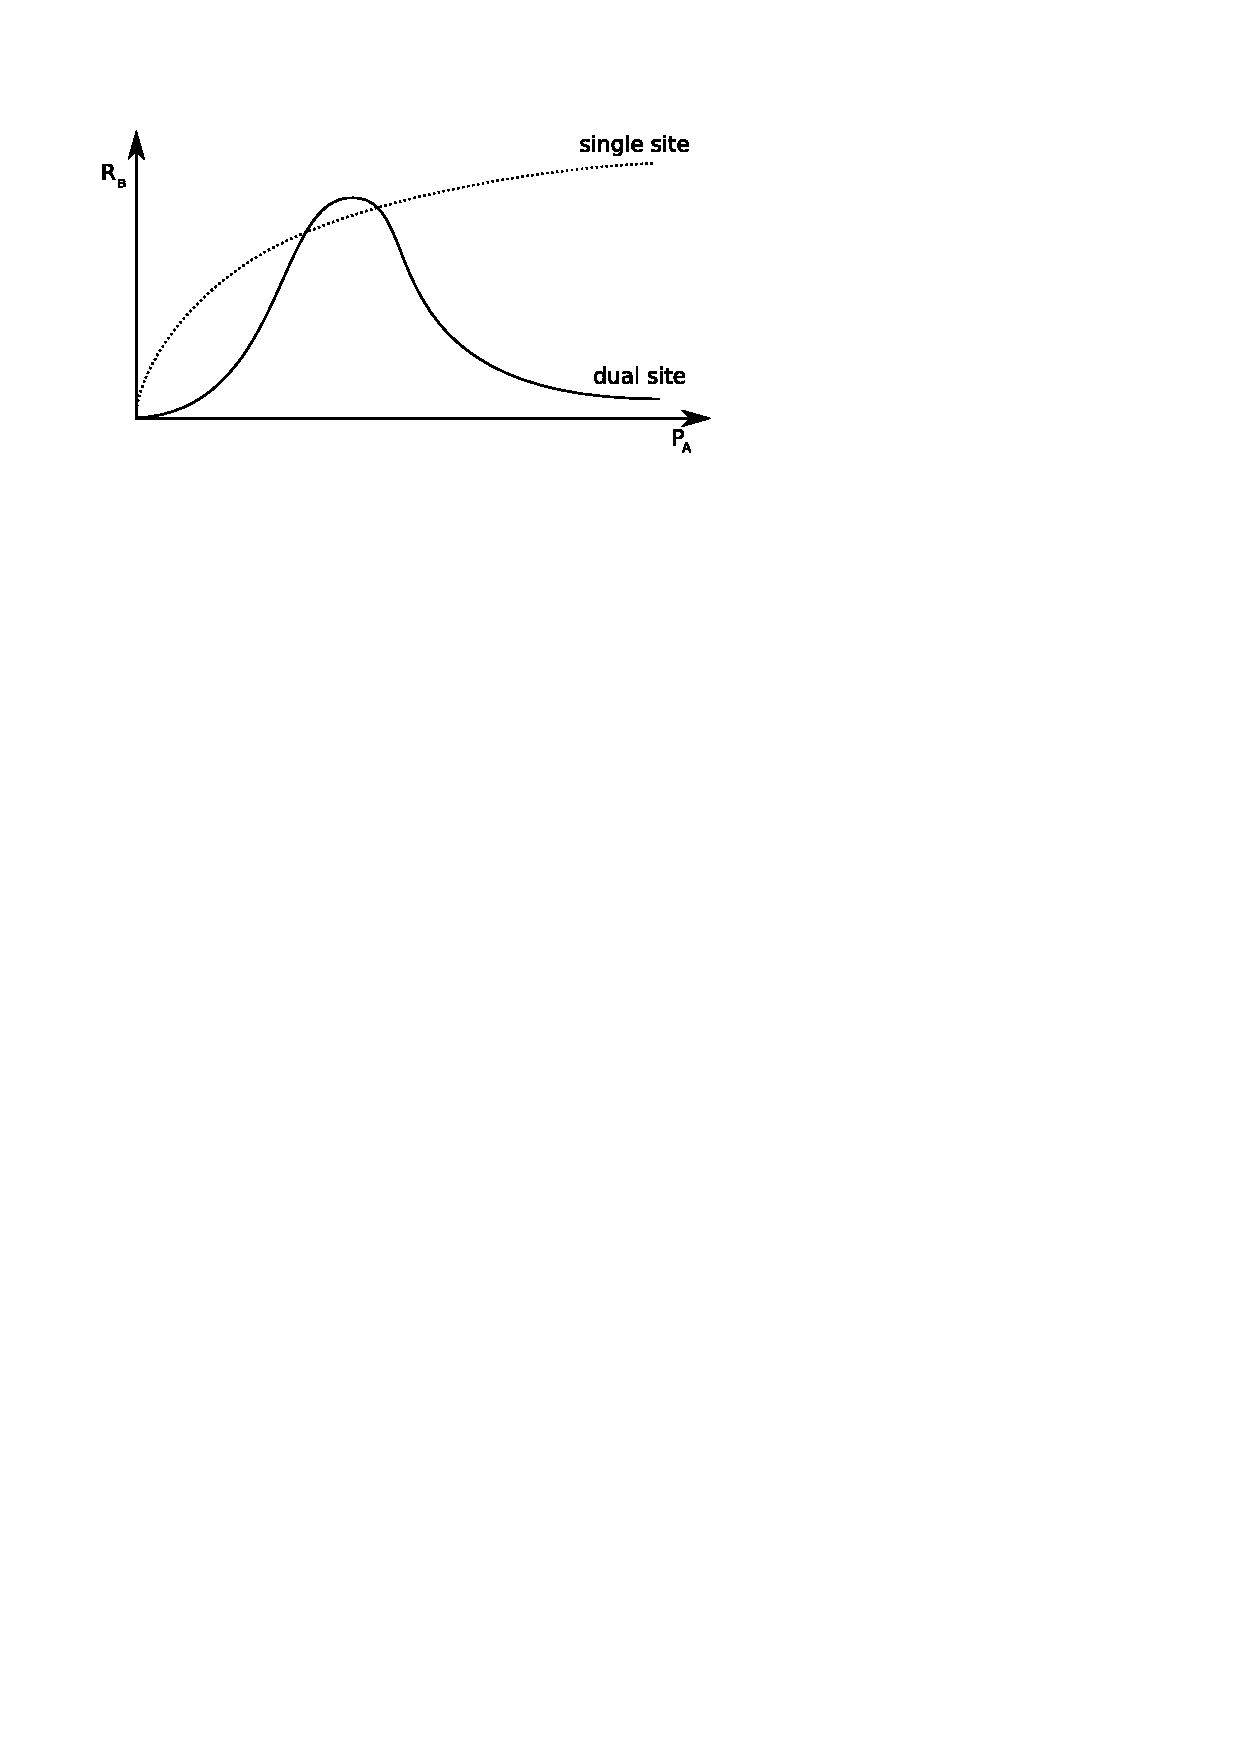
\includegraphics[width=0.50\textwidth]{image/LHHWSingleDualSite.pdf}
	\caption{Andamento della reazione secondo meccanismo \textit{single site} e \textit{dual site}.}
	\label{fig:LHHW:SingleDualSite}
\end{figure}






